\documentclass[prb,preprint]{revtex4-1} 
\raggedbottom
\usepackage{amsmath}
\usepackage{amsfonts}
\usepackage{graphicx}

\begin{document}

\title{The Measurement of the $g$-Factor for Protons in \\ Fluorine and Hydrogen Nuclei}

\author{Ryan S. Morshead, Nathan Milgram}

\affiliation{Department of Physics, California State Polytechnic University}

\date{\today}

\begin{abstract}

We utilize two oscillating magnetic fields to create achieve resonance with the protons of hydrogen and fluorine nuclei while a third field is used to produce polarized photons at frequencies which are resonant with the excited state of those protons. By identifying the frequency of the photons which are resonant with these energy states we can calculate the $g$-factor associated with these nuclei. After averaging the calculated $g$-factors for each sample containing fluorine and hydrogen nuclei, we determined our experimental result for the $g$-factor of hydrogen to be $6.010\pm0.05$ while the experimental result for the $g$-factor of fluorine was $5.620\pm0.04$. This compares to the known value for the $g$-factor of hydrogen which is $5.5857$, and the known value for the $g$-factor of fluorine which is $5.2567$. Our experimental results are unexpectedly high in both cases. The fact that the discrepancy in each case are nearly the same suggests that this error in determination occurred for all measurements independent of which sample was used. This may be due to a small bias in our experimental readout for either current or marginal oscillator frequency which would thereby cause an under estimation of the magnetic field. Alternatively improper focusing of our apparatus may have caused some distortion in the image which was observed with the spectrometer making peak measurements innaccurate.

\end{abstract}



\maketitle


\section{Introduction}

Nuclear Magnetic Resonance was first experimentally observed in late 1945, nearly simultaneously by the research groups of Felix Bloch, at Stanford University and Edward Purcell at Harvard University \cite{nobel}. The first NMR spectra were first published in the same issue of Physical Review in January of 1946. Bloch and Purcell were jointly awarded the Nobel Prize in Physics in 1952 for their discovery of Nuclear Magnetic Resonance.

The NMR phenomenon relies on the interaction of the nuclei of certain atomic isotopes with a static magnetic field\cite{NMR}. This magnetic field makes the possible spin-states of the nucleus differ in energy, and using NMR techniques the spins can be made to create observable transitions between the spin states. Common NMR active nuclei are 1H, 13C, 31P, 15N, 29Si, and many more\cite{NMR}. Nearly every element has at least one isotope that is NMR active\cite{NMR}.

Since then, NMR spectroscopy has become an indispensable tool for the determination of molecular structure, the study of molecular dynamics, and the characterization of materials at the molecular level by chemists, physicists, and molecular biologists.

This report seeks to investigate the use of NMR in determining the $g$-factor for hydrogen and fluorine nuclei while dabbling in some of it's more practical applications in chemistry and biology.

\newpage

\section{Experimental Design}

Given that protons are charged particles with spin quantum numbers of $m_s=\pm1/2$, we find that they have a magnetic moment $\mu$. Thus if placed within a magnetic field $B_0$, protons will experience energy splitting in a similar manner to electrons because they are also fermions with equal but opposite charge. However two notable differences arise when considering energy splitting in protons instead of electrons; recall that the energy of a classical magnetic moment $\mu$ in a magnetic field $B_0$ is $E=-\vec{\mu}\cdot\vec{B_0}$. As a result we write the change in energy due to splitting as 
\begin{equation}\label{Em}
E_m = \left\{
  \begin{array}{l c}
    m_s g\mu_BB_0 & \text{electrons}\\
    -m_s g\mu_NB_0 & \text{protons}
  \end{array}
\right.
\end{equation}
for electrons and protons respectively where $\mu_N$ is the nuclear magneton, $\mu_B$ is the Bohr magneton, and $g$ is what is called the ``$g$-factor". Through this expression we find two variables, $g$ and $\mu$, with unique values when calculating $E_m$ for electrons or protons. In electrons $\mu_B$ is the inherent strength of the electron's magnetic dipole moment, where an electron with a unit of angular momentum, $L$, equal to $\hbar$ would have a magnetic moment of $\mu=\mu_B$. Likewise $\mu_N$ is the inherent strength of the proton's magnetic dipole moment and would have a magnetic moment of $\mu_N$ for $L=\hbar$. The value of $g$ though is more interestingly a result of magnetic moments which are not due to the angular momentums. Through Dirac and Feynman the $g$-factor for the electron has become one of the most well known physical constants both in theory and measurement, but this is only applicable to point charges, which the proton is not. As a result the proton, a composition of three quarks, does not have a $g$-value which is known theoretically and is known solely through empirical measurement. The determination of the $g$-factor for the proton will then rely on the difference in the energy of protons with $m_s=1/2$ and $m_s=-1/2$. This energy difference can then be represented as
\begin{equation}\label{deltE}
\Delta E_{\text{proton}}= g\mu_NB_0
\end{equation}

Ultimately to make this measurement of the $g$-factor we irradiate a sample of protons with resonant photons such that they will be absorbed and cause the protons to undergo spin flips into higher energy states. Equally likely though, are stimulated emissions in which protons in higher energy states are forced into lower ones by absorbed resonant photons. In this process the incident photons are then reemitted while an additionally photon of equal energy corresponding to $\Delta E$ of the stimulated spin flip is also emitted. Those photons which are resonant will then have an energy $E_{\text{photon}}=hf_0=\Delta E_{\text{proton}}$ where $f_0$ is the resonant frequency. It should be noted that throughout this experimental procedure we will only be measuring the $g$-factor for fluorine nuclei and hydrogen nuclei. This is because of the fact that the total $m_s$ values in the nuclei sum to 1/2. If the net spins of the nuclei were larger than 1/2 there would be more than two allowable energy states. As a result one could potentially observe more than one point of resonance making it difficult to determine which frequency corresponds to which point of resonance. Additionally, since $f_0$ happens to fall between 1 MHz and 1000 MHz, we will choose to denote such frequencies as being RF or radio frequencies. Historically such frequencies are given this name because of their uses in radio and telecommunications.

It should then be recognized though, that given equal populations of protons with $m_s=1/2$ and $-1/2$ the number of photons being absorbed and emitted by the protons will be equal and thus no electromagnetic energy will be lost in the irradiation of such a system. However given a system in which unexcited $m_s=1/2$ protons are more populous there will be a net loss of electromagnetic energy which could potentially be detected in order to identify $f_0$. To determine the population inversion of protons with different spins we then use 
\begin{equation}\label{popinv}
\frac{N_2}{N_1}=\text{exp}\left(\frac{E_1-E_2}{k_BT}\right),
\end{equation}
where $N_2/N_1$ is the ratio of the number protons in higher and lower energy states, $E_1$ and $E_2$ are the energies which correspond to the respective energy states, $k_B$ is Boltzman's constant, and $T$ is the temperature of the protons. Despite the fact that at room temperature $k_BT\gg\Delta E_{\text{proton}}$ making $N_2/N_1\approx1$. Though $N_2/N_1\approx1$ the ratio is not exactly equal to 1 and thus there will be a very small but not insignificant net loss of electromagnetic energy due to the slight over population of protons in the excited state. 

To measure this net loss of energy we use a kind of $LC$ circuit called a marginal oscillator, shown in Fig \ref{LC}, to detect the effective resistance of a sample at resonance. As such, in this particular application, the circuit can be more accurately modeled as a parallel $RLC$ oscillator in parallel with a dependent current source, called the limiter. The dependent source has a nonlinear transfer characteristic based on the voltage and provides just enough current to sustain oscillation. Thus even minor increases in resistance will significantly reduce the amplitude of oscillations.

\begin{figure}[h!]
\centering
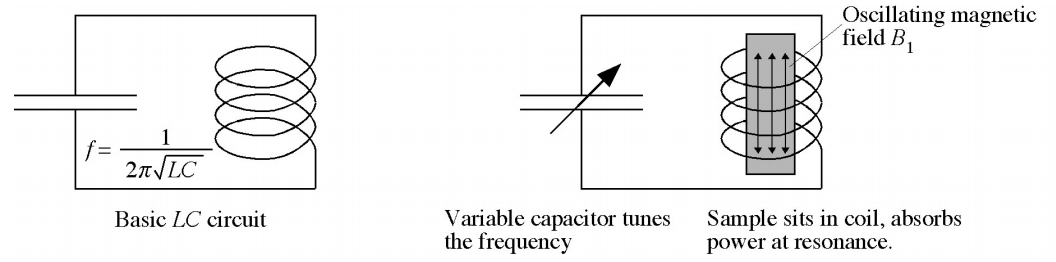
\includegraphics[width=.8\textwidth]{LC.png}
\caption{The LC circuit shown utilizes the inherent frequency of the circuit to detect minor fluctuations in the effective resistance of the sample and thus identify the point of resonance.}
\label{LC}
\end{figure}

In order to detect the net loss of electromagnetic energy in a sample of protons being irradiated with resonant photons, the sample is placed inside the solenoid of the $RLC$ circuit. By putting it there, the field $B_1$ created by the solenoid, which should be perpendicular to the field $B_0$ (responsible for energy splitting), will establish the necessary polarized photons. Then with these photons being at resonance with the excited energy state and incident on the sample, the net loss of electromagnetic energy through the absorption of photons dissipates energy from the circuit creating resistance. This along with the limiter completes the $RLC$ model described earlier thereby allowing for the identification of resonance provided the amplitude of oscillations remains marginal.

However, driving protons between the unexcited and excited states establishes a new equilibrium point where the ratio $N_2/N_1$ is no longer dependent on thermal fluctuations as shown in Eq \eqref{popinv}, but on the probability of photons to induce excitation or stimulate emissions. Given that photons are equally likely to perform either action $N_2/N_1$ would be exactly 1 causing the effective resistance of the sample to be suddenly lost at the point where the resonant photons overwhelm thermal effects. At this point it's said that the transition has been saturated. The time it takes the system to return to thermal equilibrium is the relaxation time, $T$. The magnitude of the relaxation time is a product of the interaction of the protons with the magnetic moments of the lattice nuclei and is called the spin-lattice interaction. Though the term ``lattice nuclei" is not particularly indicative of materials which are not solids similar interactions seen in liquids, like the ones used in this report, are still defined as spin-lattice interactions.

To compensate for saturation, we include a third magnetic field, $B_\text{mod}$ whose purpose is to modulate $B_1$ about the resonant frequency at a pace which allows thermal fluctuations to return to prevalence after each pass over resonance. As a result the resonant frequency can be achieved while the frequency of the field $B_1$, $f_\text{RF}$, does not equal $f_0$ as long as the amplitude of the modulation $A_{f_\text{mod}}$ is large enough. In order to identify $f_0$ without an error of $\pm A_{f_\text{mod}}$ we ensure that the time between each observed pass over $f_0$ is the same, implying that the frequency of the field $f_\text{RF}$, equals $f_0$. Thus in knowing $f_\text{RF}$ at the point where resonance occurs at equal intervals, $f_0$ is known. Then with $B_0$ known, it's useful to show that by combining Eq \eqref{deltE} with the expression $E_{\text{photon}}=hf_0=\Delta E_{\text{proton}}$ we can solve for $g$ in terms of $B_0$ and $f_0$ in the form
\begin{equation}\label{g}
g=\frac{hf_0}{\mu_NB_0}.
\end{equation}

The exact arrangement of the magnetic fields $B_0$, $B_1$, and $B_\text{mod}$ which was used to make the required measurements of these fields and their respective frequencies is shown in Fig \ref{expfig}.
\begin{figure}[h!]
\centering
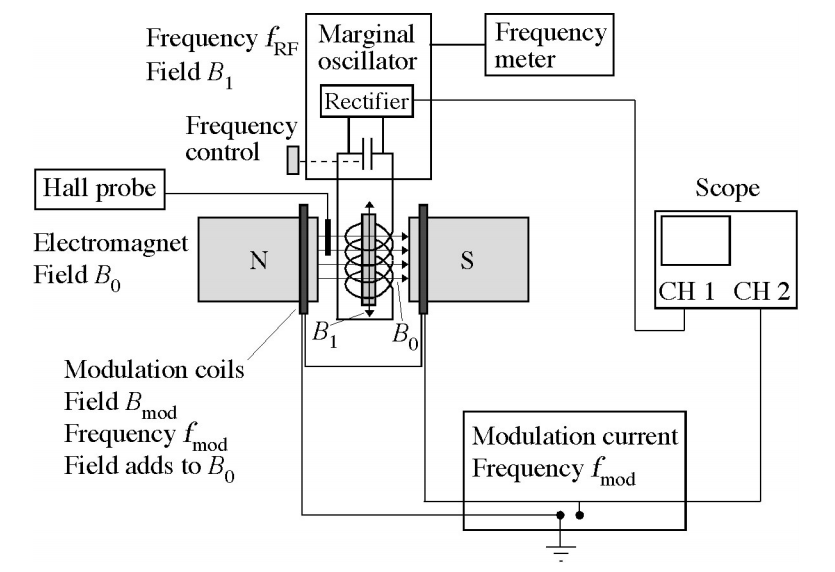
\includegraphics[width=.8\textwidth]{expfig.png}
\caption{Experimental arrangement.}
\label{expfig}
\end{figure}

\newpage

\section{Results and Analysis}

In order to determine the strength of the magnetic field $B_0$ our samples were exposed to, a calibration was performed to determine the relationship between the current provided to the electromagnet and the resulting magnetic field. This data was then separated into two distinct data sets with separate calibration equations; one was linear while the other was of the form of a second order polynomial. The raw data along with the calibration curve fits are shown in Fig \ref{magcal} and \ref{magcal1}.

\begin{figure}[h!]
\centering
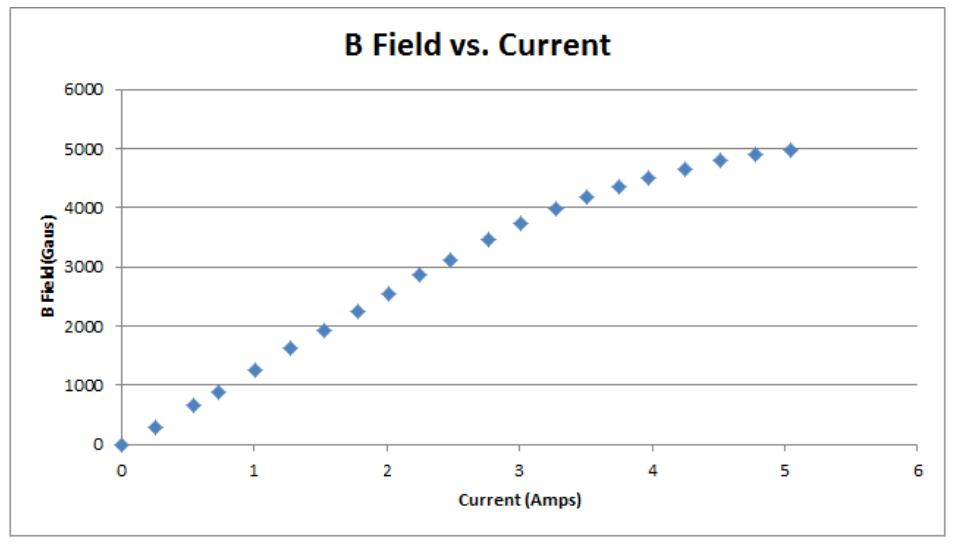
\includegraphics[width=.8\textwidth]{magcal.png}
\caption{asdasd}
\label{magcal}
\end{figure}

\begin{figure}[h!]
\centering
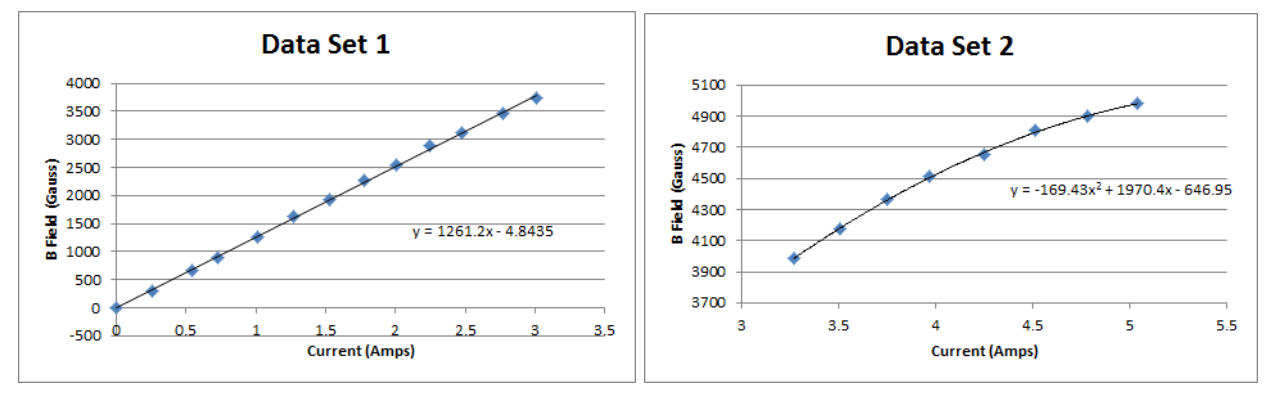
\includegraphics[width=.8\textwidth]{magcal1.png}
\caption{asdasd}
\label{magcal1}
\end{figure}

From this calibration, we were able to determine the magnetic field supplied by an arbitrary current. After measuring the resonant frequency and the magnetic field $B_0$, the $g$-factor could be calculated using Eq \ref{g}. We then began comparing pure water to a solution of copper sulfate. Our target for these two samples was the hydrogen nuclei present in the water. After averaging our results we find that the $g$-factor for water was 5.98$\pm0.04$ while our g factor for the copper sulfate solution was 6.04$\pm0.05$. It should be noted that the copper sulfate solution had a much stronger resonance signal than the pure water. This is because of a process called the spin lattice interactions during which the relaxation time decreases in the coper solution.

Samples of Glycerine, Polystyrene, and Polytetraflourethylene (PTFE) were analyzed, and again our target for these samples was the hydrogen nuclei with the exception of PTFE which targets fluorine nuclei. Here we found that the $g$-factor were 6.01$\pm0.05$, 5.980$\pm0.04$, and 5.620$\pm0.04$ respectively. The signal for PTFE was observed to have a single, relatively wide peak. The peak's full width at half maximum was measured by determining the tick mark to frequency relationship which was 20$\times10^{-4}$ MHz per division on the oscilloscope. The peak's full width at half maximum was then determined to be 9$\pm1\times10^{-4}$ MHz.

In order to observe the potential applications of NMR in chemistry, a sample of hand lotion was analyzed. The $g$ factor for the lotion was determined to be 5.970$\pm0.04$. In comparing this result with the data described earlier, the $g$ factor for the lotion more closely resembles the sample of glycerine, suggesting that the lotion contains glycerine.

Finally, samples of celery, carrot, and glycerine were analyzed in order to observe the potential applications of NMR in biology. The $g$ factor for the celery was determined to be 5.98$\pm0.04$, it was 6.01$\pm0.05$ for carrots, and 6.0$\pm0.3$ for glycerine. The results for celery and carrot, upon inspection, closely resemble our water sample, which suggests, as expected, that our biological samples contain mostly water. Glycerine on the other had is also surprisingly similar to water and may be due to the fact that they share a similar composition.

As an aside, the question of how much a water soluble contaminant would affect results was analyzed. To answer it solutions of lotion, salt, hot sauce and jam were analyzed. It was found that the $g$-factor of water with the contaminants was $6.05\pm0.05$, $5.98\pm0.04$, $5.97\pm0.04$, and $6.00\pm0.04$ respectively. These findings would suggest that contaminants have a noticeable effect on our data. It is also apparent that certain contaminants are more repercussive to our data than others. The glycerine from the lotion and the sugar from the jam seem to have had a significant effect on the data, while the sodium from the hot sauce and salt seem to have been relatively inconsequential, but not unnoticeable.

\newpage

\section{Conclusion}

In averaging the calculated $g$-factors for each uncontaminated sample, we determine our experimental result for the $g$-factor of hydrogen to be $6.01\pm0.05$. From the PTFE sample, the experimental result for the $g$-factor of Fluorine is $5.62\pm0.04$. This compares to the known value for the $g$-factor of hydrogen which is $5.5857$, and the known value for the $g$-factor of fluorine which is $5.2567$. Our experimental results are unexpectedly high in both cases. The fact that the discrepancy in each case are nearly the same suggests that this error in determination occurred for all measurements independent of which sample was used. This may be due to some experimental malpractice, possibly a faulty calibration. It is also possible that there was a small bias in our experimental readout for either current or marginal oscillator frequency. It is also possible that we experienced some small bias in our experimental readout for either current or marginal oscillator frequency.

\newpage

\begin{acknowledgments}

Thank you to my esteemed colleagues who agreed with me when I proposed more large explosions in the report as an answer to its technical flaws. Though my editor would not allow the changes I acknowledge their support.

\end{acknowledgments}


\begin{thebibliography}{99}

\bibitem{nobel} ``The Nobel Prize in Physics 1952". Nobelprize.org. Nobel Media AB 2013. Web. 3 Feb 2014. http://www.nobelprize.org/nobel\_prizes/physics/laureates/1952/.

\bibitem{NMR} Hornak, J. P. (1996). The basics of nmr. (1st ed.). Rochester, New York: Rochester Institute of Technology

\end{thebibliography}

\end{document}